\section{Kommunikation}
\label{src:kommunikation}
Eine unserer größten Aufgaben als \glqq{}Simulations-Gruppe\grqq{} bestand neben der Programmierung und Implementierung einer funktionierenden und benutzerfreundlichen Simulation in der Kommunikation und Vermittlung mit den anderen Gruppen des Praktikums. Insbesondere erwähnt seien hier die \glqq{}Arduino-Gruppe\grqq{}, denen unsere Simulation als Basis dienen sollte und der \glqq{}Bezierkurven-Gruppe\grqq{}, welche die für uns benötigten Winkelsequenzen aus einer Menge von Bezierkurven extrahierten. 

\subsection{Der Input für unsere Simulation}
\label{sec:input}
Zu Beginn des Programmierpraktikums stellte sich uns vor allem die Frage nach den Input-Daten, welche wir bekommen und dann im Sinne einer Simulation weiterverarbeiten sollten. Recht schnell wurde uns klar, dass wir mit der reinen Implementation einer voll­um­fäng­lichen Simulation schon gut beschäftigt sein würden. Deshalb einigten wir uns darauf, dass die Aufgabe, aus den gegebenen Bezierkurven  Winkelsequenzen zu erstellen, nicht bei uns liegen sollte, sondern eine Aufgabe der Gruppe vor uns darstellt. Die Idee hinter der Nutzung dieser Sequenzen als Input war, dass wir mit denselben, sehr hardwarenah gedachten, Größen operieren, welche auch der Arduino später bekommen sollte. Da die Winkelsequenzen direkt die Motoren steuern, erschien uns das hier am sinnvollsten. \\
Wir wollten unsere Simulation von Beginn an so anpassungsfähig wie möglich gestalten, dazu haben wir uns recht schnell auf eine externe Text-Datei mit den oben erwähnten Winkelsequenzen geeinigt. Diese konnten dann später sowohl von unserer Simulation, als auch (per SD-Karte) vom Arduino selbst eingelesen werden, was uns ermöglichte, sehr flexibel und schnell zwischen verschiedenen zu zeichnenden Formen zu wechseln. Um ein möglichst realitätsnahes Ergebnis zu erreichen, wurde uns zudem pro Winkelsequenz ein diskreter Zeitwert in Millisekunden gegeben, in dem der Arduino diese Winkelsequenz abarbeitet. Zudem wurde nach dem ersten Praxis-Test mit dem Arduino am Whiteboard klar, dass es (auch zur Bemessung der Zeichenungenauigkeiten) hilfreich wäre, eine Winkelsequenz von einem von uns definierten Startpunkt zu dem wirklichen Zeichenstartpunkt des Bildes und zurück zu haben. Nach Besprechung mit den Tutoren haben wir uns darauf geeinigt, die erste Zeile einer Datei zu verwenden, um zum Zeichenstartpunkt zu kommen und die zweite Zeile, um wieder zum Anfangspunkt zu gelangen. Die folgenden Winkelsequenzen werden dann dazu genutzt, das eigentliche Bild zu zeichnen. Unsere Abmachung war es, dass positive Winkel immer mehr Schnur geben, während negative die Schnur verkürzen. \\
In der folgenden Grafik ist dieses Format einer .txt-Datei schematisch abbgebildet: \\

\begin{figure}[ht]\centering
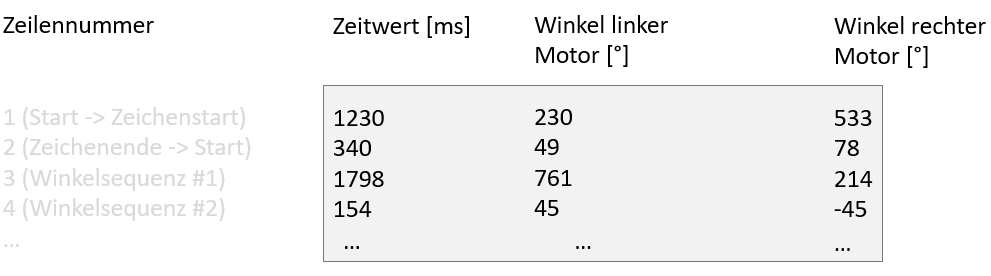
\includegraphics[width=\linewidth]{images/dateiformat.png}
\caption{Schematische Darstellung einer .txt Datei im festgelegten Format}
\label{fig:dateiformat}
\end{figure}

\subsection{Fehlererkennung}
Allgemein hat die kontinuierliche Absprache mit den anderen Gruppen sehr dabei geholfen, sowohl eigene Fehler in unserer Simulation, als auch Fehler bei Anderen zu entdecken. \\
So half unsere Simulation bei dem ersten \glqq{}Praxis-Test\grqq{}, wo wir mittels des Arduinos auf einem Whiteboard gezeichnet haben, mit einem verstellbaren Slider für den Spulendurchmesser (s. Section \ref{sec:paras}) Unklarheiten bezüglich diesen zu klären.\\
Auch haben wir erkannt, dass es wesentliche Missverständnisse bezüglich des Koordinatenursprungs gegeben hatte: So hatte eine Gruppe diesen unten links gewählt, während andere Gruppen aber von oben links ausgegangen sind. Das hat zu falschen Endergebnissen und Diskrepanz zwischen den zu erwartenden Ergebnissen und denen unserer Simulation geführt. \\
Der letzte große Fehler, der zu  einem falschen Endergebnis innerhalb der Simulation geführt hatte, lag allerdings bei uns: Wir hatten durch unsere Algorithmen dafür gesorgt, dass das gezeichnete Bild auch wirklich kontinuierlich ist und nicht etwa nur jeder Endpunkt einer Winkelsequenz gemalt wird. Hier ist es uns aber durch diverse Logikfehler (dazu schreibt Lino mehr) passiert, dass sich der wirkliche Endpunkt (hätten wir direkt die vollen Winkel einer Sequenz genommen) von dem unseren Programms unterschied. \\
Alle oben genannten Fehler konnten wir als Gruppe und mithilfe der Tutoren gut beheben, sodass wir am Ende des Praktikums die von uns ausgesuchten Bilder erkennbar zeichnen konnten. \\